 \chapter{$H_\infty$ design for robust control}

\section{Robust control via classical loop-shaping}
First , we consider the problem of designing a robust controller $G_c$ by means of classical loop shaping techniques. To this aim we present a set of necessary and sufficient conditions for robust performance fulfillment in terms of the frequency response of the loop function $L(s)$. Some general guildlines are provided about the design of a controller $G_c$ which provides the desired shape of the loop function. Our attention is restricted to the case of $W_T = 0$.\\


The following result provides \textbf{necessary conditions} for \textbf{robust performance} fulfillment in terms of the frequency response of the loop function $L(s)$.\\

\subsection{Result (Necessary conditiono for the case $|W_u|< 1$)}

Assume that $|W_u| < 1$. If the feedback system is such that 
\[
\||W_sS_n|+|W_uT_n|\|_\infty < 1
\]
Then, the loop function satisfies the following constraints:
\[
|L(j\omega)| > \frac{|W_s(j\omega)|-1}{1 - |W_u(j\omega)|} \:\:\forall \:\: \omega
\]

\textbf{Remark:} $|W_u| < 1$ is usually satisfied only at low frequencies.\\

\subsection{Result (Necessary conditiono for the case $|W_S|< 1$)}
Assume that $|W_S|<1$. If the feedback system is such that \\
\[
\||W_SS_n|+|W_uT_n|\|_\infty < 1
\]
then the loop function satisfied the following constraints
\[
|L(j\omega)| < \frac{1-|W_s(j\omega)|}{|W_u(j\omega)|-1} \:\:\forall \:\: \omega
\]
\textbf{Remark:} $|W_S| < 1$ is usually satisfied only at high frequencies.\\

he following result provides \textbf{sufficient conditions} for \textbf{robust performance} fulfillment in terms of the frequency response of the loop function $L(s)$.\\


\subsection{Result (Suffiecient conditiono for the case $|W_u|< 1$)}

Assume that $|W_u| < 1$. If the loop function satisfied the following constraints
\[
|L(j\omega)|> \frac{|W_S(j\omega)|+1}{1-|W_u(j\omega)|} \:\:\: \forall \:\:\: \omega
\]
then the feedback system is such that 
\[
\||W_SS_n|+|W_uT_n|\|_\infty < 1
\]

\textbf{Remark:} Again $|W_u| < 1$ is usually satisfied only at low frequencies.\\


\subsection{Result (Sufficient conditiono for the case $|W_S|< 1$)}
Assume that $|W_S|<1$. If the feedback system is such that \\
then the loop function satisfied the following constraints
\[
|L(j\omega)| < \frac{1-|W_s(j\omega)|}{|W_u(j\omega)|-1} \:\:\forall \:\: \omega
\]
then the feedback system is such that 
\[
\||W_SS_n|+|W_uT_n|\|_\infty < 1
\]

\textbf{Remark:} Also in this case, $|W_S| < 1$ is usually satisfied only at high frequencies.\\

\subsection{conclusion}
Since typical shapes of $W_S$ and $W_u$ are such that:
\[
|W_S(j\omega)| \gg 1  \text{  at low frequency}
\]
\[
|W_u(j\omega)| \gg 1  \text{  at high frequency}
\]

the following 
\[
|L(j\omega)| > \frac{W_S(j\omega)}{1- |W_u(j\omega)|}
\]
is a \textbf{necessary and sufficient condition at low frequency}, and

the following 
\[
|L(j\omega)| < \frac{1- W_S(j\omega)}{|W_u(j\omega)|}
\]
is a \textbf{necessary and sufficient condition at high frequency}.

 \begin{figure}[H]
    \centering
    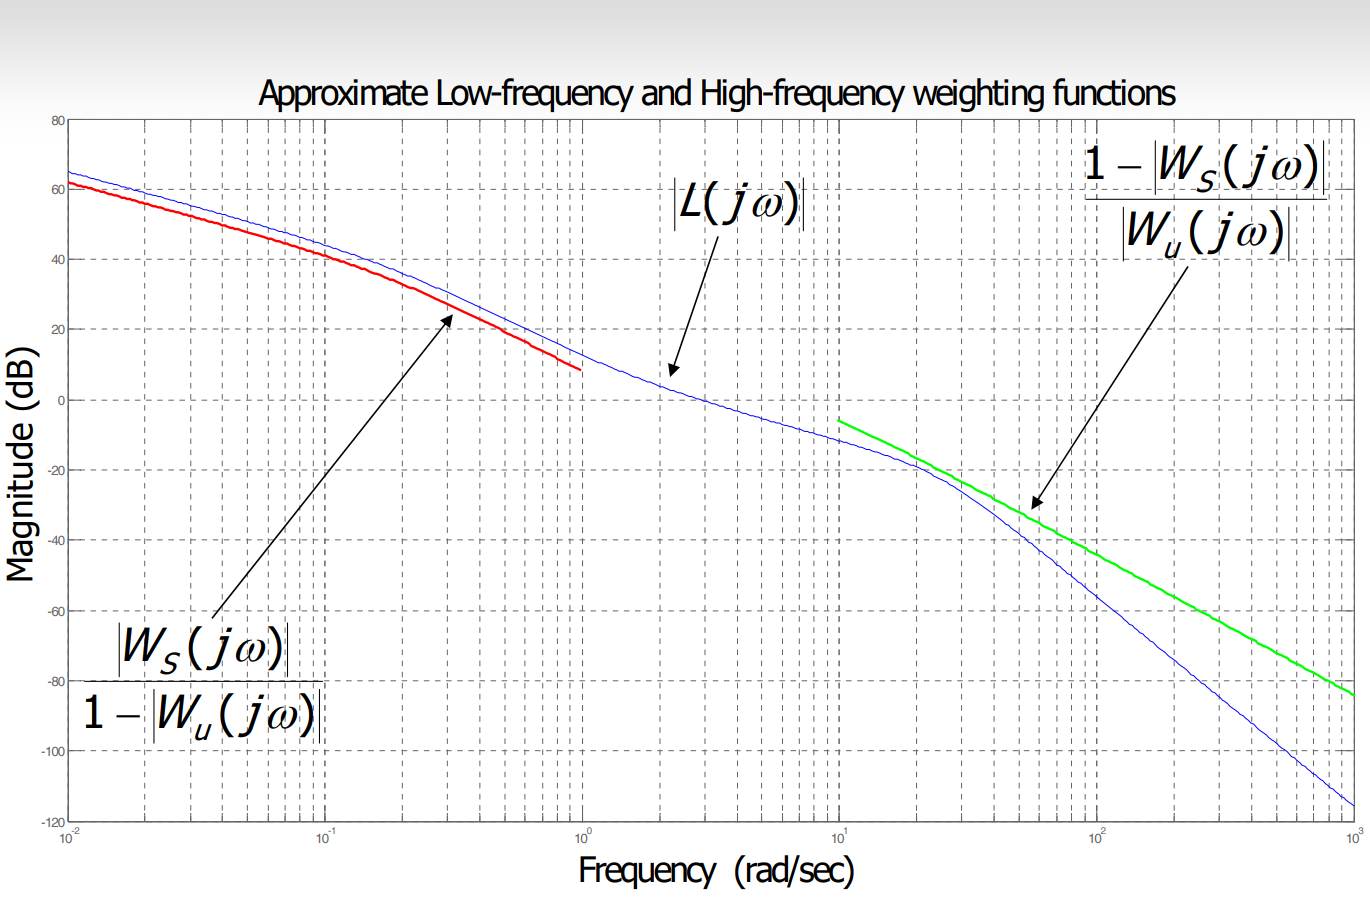
\includegraphics[width=0.75\textwidth]{robust-loop-shaping.png}
    \caption{Robust performance condition in the context of classical loop shaping.}
 \end{figure}

The obtained necessary and sufficient conditions provide traints on the magnitude of  the loop function at low and high frequencies.\\

As to the frequency range in the neighborhood of $\omega_c$, the loop function must be shaped in such a way to guarantee good stability.\\

\subsection{Controller design guidelines}
\begin{itemize}
    \item Select $\omega_c$ on the basis of the transient response requirements and the high and the low frequency range constraints on the magnitude of $L$.
    \item Select the gain $K_c$ and the number of poles of $G_c$ at $s=0$ in such a way as to satisfy the low frequency range constraints on the magnitude of $L$.
    \item Add the required lead/lag networks to satisfy the constraints related to the desired value sof $T_p$ and $S_p$ (the Nichols chart might help).
\end{itemize}

\section{Robust control via $H_\infty$ norm minimization}


First of all, let us recall the definition of he $H_\infty$ norm of a SISO LTI system with transfer function $H(s)$:
\[
\|H(s)\|_\infty = \max\limits_{\omega} |H(j\omega)|
\]
While the definition of the $H_\infty$ norm of a MIMO LTI system with transfer function $G(s)$ is:
\[
\|G(s)\|_\infty = \max\limits_{\omega} \bar{\sigma}(G(j\omega))
\]
where $\bar{\sigma}$ is the maximum singular value of $G(j\omega)$ for all $\omega$
This is the definition of the generalized norm. In the MATLAB, the command \texttt{norm(G,inf)} should be used.

\textbf{A different approach is presented now, where the controller $G_c$ is obtained by solving a suitable optimization problem.}\\

We consider general control problem where:
\begin{itemize}
    \item The plant is described by means of one of the four unstructured uncertainty model sets (additive, multiplicative, inverse additive, inverse multiplicative)
    \item  The norm performance requirements lead to the following conditions
    \[
    \|W_SS_n\|_\infty < 1 \hspace{1cm} \|W_TT_n\|_\infty<1
    \]
\end{itemize}

The $H_\infty$ norm minimization approach, called $H_\infty$ control, refers to a general formulation of the control problem which is based on the following block diagram representation of a general feedback system.

 \begin{figure}[H]
    \centering
    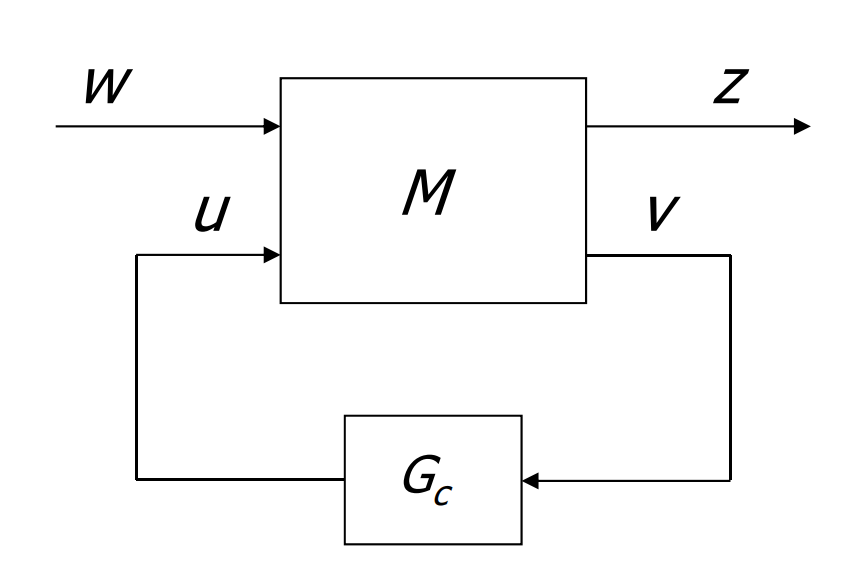
\includegraphics[width=0.5\textwidth]{gc-generalized-plant.png}
    \caption{The generalized plant considered for the control problem in the $H_\infty$ context.}
 \end{figure}
 
Where $M$ is the \textbf{generalized plant}, $G_c$ is the controller, $u$ is the vector of control inputs, $v$ is the vector of controller inputs, $w$ is the vector of external inputs, $z$ is the vector of external outputs, which can be used for the minimization of desirable criteria. \\

The external input and output signals of the generalized plant are not necessarily physical variables of the control system. The external input and output signals of the generalized plant must be carefully selected in order to take into account the stability/performance requirements of the considered control problem.\\

In the $H_\infty$ design, the controller is obtained by solving the following optimization problem
\[
G_c(s) = \arg \min\limits_{G_c \in G_c^{stab}} \|T_{wz}(s)\|_\infty
\]
$G_c^{stab}$ is the class of all the controllers which provide internal stability of the nominal feedback system.\\

$T_{wz}$ is the closed loop transfer function between the input $w$ and the output $z$

As previously stated, in $H_\infty$ control the controller $G_c$ is designed by minimizing the $H_\infty$ norm of the function $T_{wz}$.\\

Therefore, the key step is the proper selection of the generalized plant $M$ which must be build taking into account all the requirements of the considered control problem.\\

The design of the controller is performed in three steps:
\begin{itemize}
    \item select the transfer function $T_{wz}$
    \item build the generalized plant $M$ conrresponding the selected transfer function $T_{wz}$, which is the transfer function from the input $w$ to the output $z$.
    \item compute $G_c(s)$ by solving the optimization problem
    \[
    G_c(s) = \arg \min\limits_{G_c \in G_c^{stab}} \|T_{wz}(s)\|_\infty
    \]
    where as it was explained, $G_c^{stab}$ is the set of all the controllers which provide internal stability of the nominal feedback system.
\end{itemize}

If we find a controller $G_c$ that minimezes $W_uT_n$ and the result becomes less than 1 for all the frequencies, then the resultant controller is going to guarantee robust stability. Now, the question is that how to select $T_{wz}$?
\section{Generalized Plant for Robust Stability}
Now, let us consider the problem of designing a controller $G_c$ to robustly stabilize an uncertain system described by the unstructured multiplicative model set:
\[
M_m = \left\{G_p(s) = G_{pn}(s)[1 + W_u(s)\Delta(s)],\,\|\Delta(s)\|_\infty \leq 1\right\}.
\]
The condition for robust stability is known to be:
\[
\|W_uT_n\|_\infty < 1.
\]
In this case, we design a controller $G_c$ to minimize the weighted $H_\infty$ norm of a single transfer function. If the achieved minimum is less than 1, then the obtained controller robustly stabilizes the uncertain system.

The condition for robust stability is:
\[
\|W_uT_n\|_\infty < 1.
\]
The problem of designing a controller $G_c$ to satisfy the robust stability condition for unstructured multiplicative uncertainty can be solved by choosing the following transfer function $T_{wz}$:
\[
T_{wz}(s) = W_2T_n,
\]
where:
\[
W_2(s) = W_u(s).
\]
Assume, without loss of generality, that $G_f = G_s = G_a = 1$. The generalized plant $M$ corresponding to the selected transfer function $T_{wz}$ is the following (the portion inside the dashed box).

\begin{figure}[H]
    \centering
    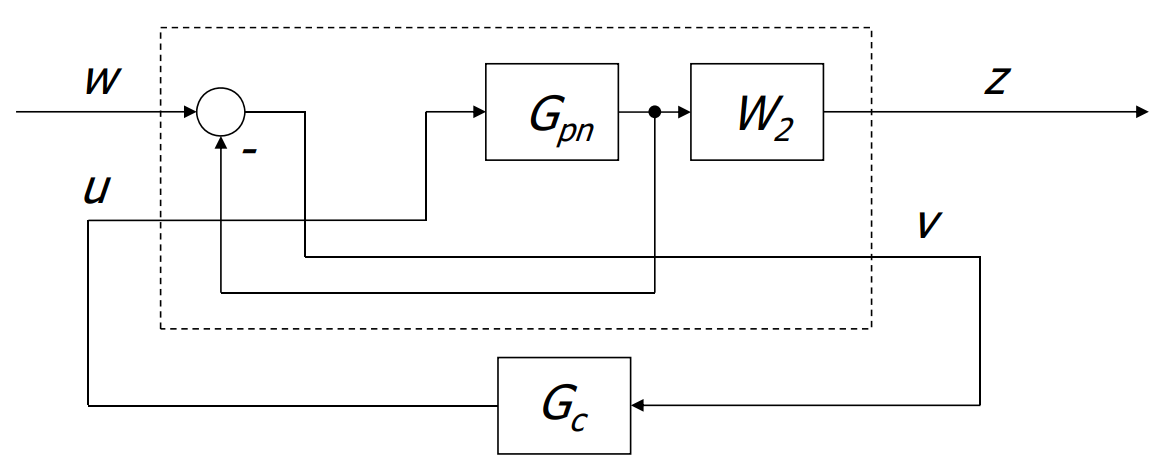
\includegraphics[width=0.75\textwidth]{gc-generalized-plant-robust-stability.png}
    \caption{The generalized plant considering the structure of our problem in the $H_\infty$ context.}
\end{figure}

\section{Generalized Plant for Nominal Performance}
Now, let us consider the problem of designing a controller $G_c$ to satisfy nominal performance:
\[
\|W_SS_n\|_\infty < 1, \hspace{0.5cm} \|W_TT_n\|_\infty < 1.
\]
\textbf{In this case, the goal is to design a controller $G_c$ that minimizes both of these weighted $H_\infty$ norms.} If the achieved minimum is less than 1, then the obtained controller satisfies the assigned nominal performance requirements.

To achieve this objective, we exploit the following result on the $H_\infty$ norm of a stack of transfer functions:

\subsection{Result (Norm of a Stack of Transfer Functions)}
\[
\left\|
\begin{array}{c}
H_1 \\
H_2 \\
\vdots \\
H_i \\
\vdots \\
H_n
\end{array}
\right\|_\infty
< 1
\implies
\|H_i\|_\infty < 1, \quad \forall i.
\]
According to this result, the minimization of the $H_\infty$ norm of $n$ transfer functions can be performed by minimizing the $H_\infty$ norm of the stack of such transfer functions ("stacking procedure").

\subsection{Result (Conservativeness of the Stacking Procedure)}
\[
\|H_i\|_\infty = 1 \quad \forall i \implies 
\left\|
\begin{array}{c}
H_1 \\
H_2 \\
\vdots \\
H_i \\
\vdots \\
H_n
\end{array}
\right\|_\infty
= \sqrt{n}.
\]
This result shows that the $H_\infty$ norm of a stack of transfer functions is (in the worst case) $\sqrt{n}$ times the value of the $H_\infty$ norm of each single transfer function.

Thus, the problem of designing a controller $G_c$ to satisfy the following nominal performance conditions:
\[
\|W_SS_n\|_\infty < 1, \hspace{0.5cm} \|W_TT_n\|_\infty < 1,
\]
can be solved by choosing the following transfer function $T_{wz}$:
\[
T_{wz} =
\begin{bmatrix}
W_1S_n \\
W_2T_n
\end{bmatrix},
\]
where:
\[
W_1(s) = W_S(s), \quad W_2(s) = W_T(s).
\]

\begin{figure}[H]
    \centering
    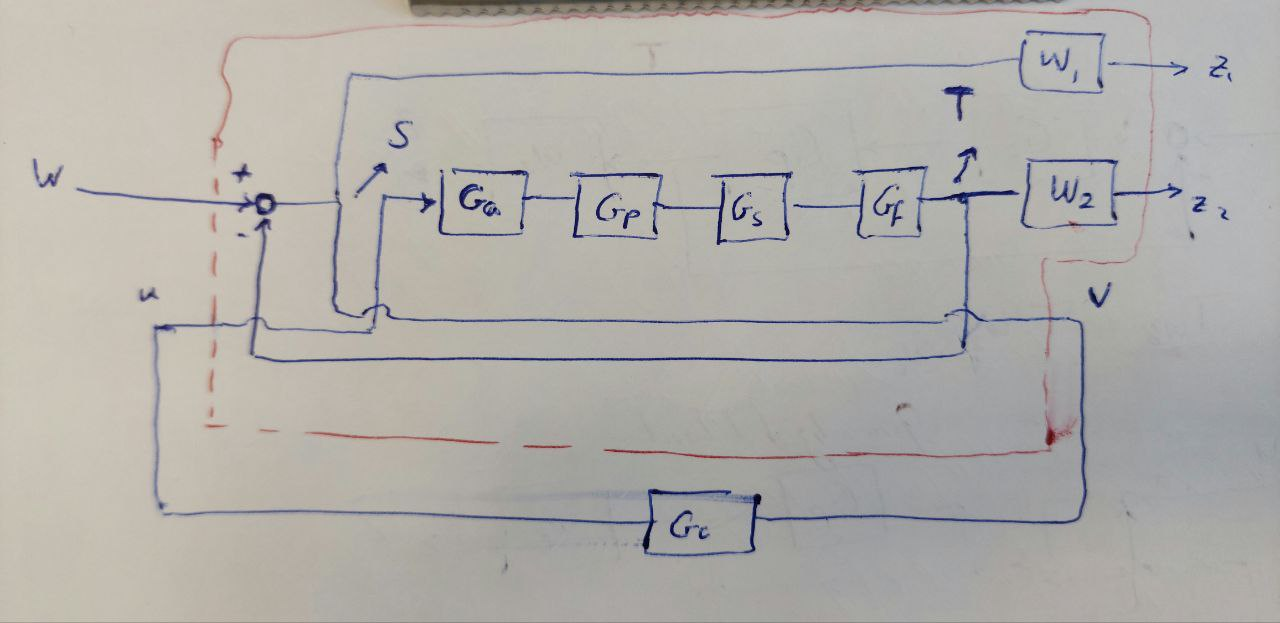
\includegraphics[width=0.5\textwidth]{gc-generalized-plant-2.jpg}
    \caption{The generalized plant considering the structure of our problem in the $H_\infty$ context.}
\end{figure}

\section{Generalized Plant for Nominal Performance (NP) and Robust Stability (RS)}
Finally, let us consider the problem of designing a controller $G_c$ to satisfy \textbf{both} nominal performance and robust stability conditions. In this case, the controller $G_c$ must be such that:
\[
\|W_SS_n\|_\infty < 1, \hspace{0.5cm} \|W_TT_n\|_\infty < 1, \hspace{0.5cm} \|W_uT_n\|_\infty < 1.
\]

The complementary sensitivity function must satisfy the following frequency domain constraints:
\[
|T_n(j\omega)|\leq|W_T^{-1}(j\omega)|,\quad |T_n(j\omega)|\leq|W_u^{-1}(j\omega)|, \quad \forall \omega.
\]

Thus, the problem of designing a controller $G_c$ which robustly stabilizes the given uncertain system and fulfills the nominal performance requirements can be solved by choosing the following transfer function $T_{wz}$:
\[
T_{wz} =
\begin{bmatrix}
W_1S_n \\
W_2T_n
\end{bmatrix},
\]
where \( W_1(s) = W_S(s) \) and \( W_2(s) \) is such that for each \(\omega\):
\[
|W_2(j\omega)| = \max(|W_u(j\omega)|,\,|W_T(j\omega)|).
\]

\begin{figure}[H]
    \centering
    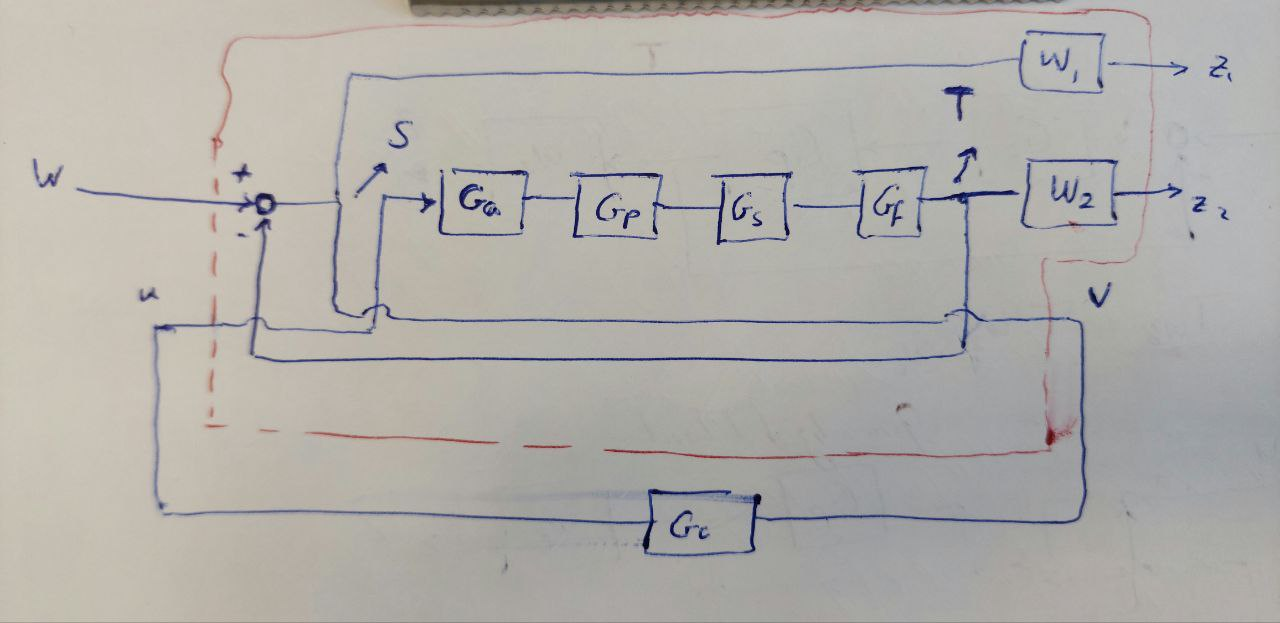
\includegraphics[width=0.5\textwidth]{gc-generalized-plant-2.jpg}
    \caption{The generalized plant considering the structure of our problem in the $H_\infty$ context.}
\end{figure}

Control problems involving constraints on the $H_\infty$ norm for more than one closed-loop transfer function are called \textbf{mixed sensitivity problems}. Examples include:
\begin{itemize}
    \item Designing $G_c$ to fulfill nominal performance requirements, leading to $H_\infty$ norm constraints on both $S_n$ and $T_n$.
    \item Designing $G_c$ to fulfill both nominal performance and robust stability requirements. (For this problem look at the last chapter of the book Doyle).
\end{itemize}

The controller design problem obtained by applying the \textbf{stacking procedure} to a mixed sensitivity problem is referred to as a \textbf{stacked mixed sensitivity problem}.

 \section{$H_\infty$ control: LMI optimizatino approach}
 As previously stated in the $H_\infty$ control, the controller is designed by solving the following optimization problem:
 
 \[
 G_c(s) = \arg \min\limits_{G_c \in G_c^{stab}} \|T_{wz}(s)\|_\infty
 \]
 
 Among the approaches proposed in the literature which solve such an optimization problem, we exploit the one based on the solution of a suitable constrainted optimization problem where the constraints are in the form of \textbf{Linear Matrix Ineqaulities} (LMI).\\
 
 The LMI based approach is implemented in the MATLAB LMI constrol system toolbox.\\
 
The LMI approach is based on a state-space description of the generalized plant $M$, which is depicted in the following figure:
The scheme of the generalized plant is as follows:
\begin{figure}[H]
    \centering
    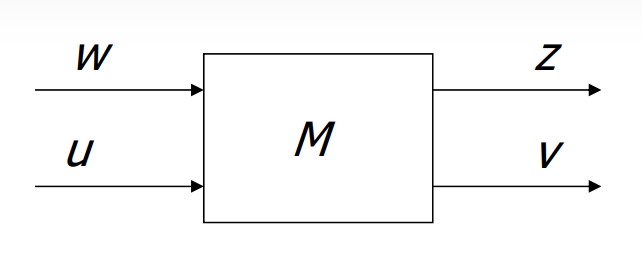
\includegraphics[width=0.5\textwidth]{generalized-plant.png}
    \caption{The scheme of the generalized plant.}
\end{figure}

\[
M: 
\begin{cases}
\dot{x}_M = A x_M + B_1 w + B_2 u\\
z = C_1 x_M + D_{11} w + D_{12} u\\
v = C_2 x_M + D_{21} w + D_{22} u
\end{cases}
\]

where \textbf{$x_M$ is the state vector of the generalized plant.} 

Referring to the mixed sensitivity problem, we have that:
\begin{itemize}
\item $x_M$ is given by the union of the state variables of the nominal model $G_{pn}$ and those of the weighting functions $W_1$ and $W_2$.
\item the eigenvalues of matrix $A$ are the union of the poles of the transfer functions $G_{pn}$, $W_1$, and $W_2$.
\end{itemize}

For the sake of simplicity and without loss of generality, assume that the controller $G_c$ to be designed is a SISO system (i.e. $u$ and $v$ are scalar signals).\\

The LMI optimization problem can be solved under the following mild assuptions:
\begin{itemize}
    \item[I] the matrix triplet ($A$,$B_2$,$C_2$) is stabilizable (i.e. if all unstable modes are controllable) and detectable (i.e. if all unstable modes are observable)
    \item[II] $D_{22} = 0$
\end{itemize}

Now, we will discuss the implementations of assumptions I and II on the solution of the mixed sensitivity problem. To this aim, let us consider again the generalizeed plant for the mixed sensitivity problem. 

\begin{figure}[H]
    \centering
    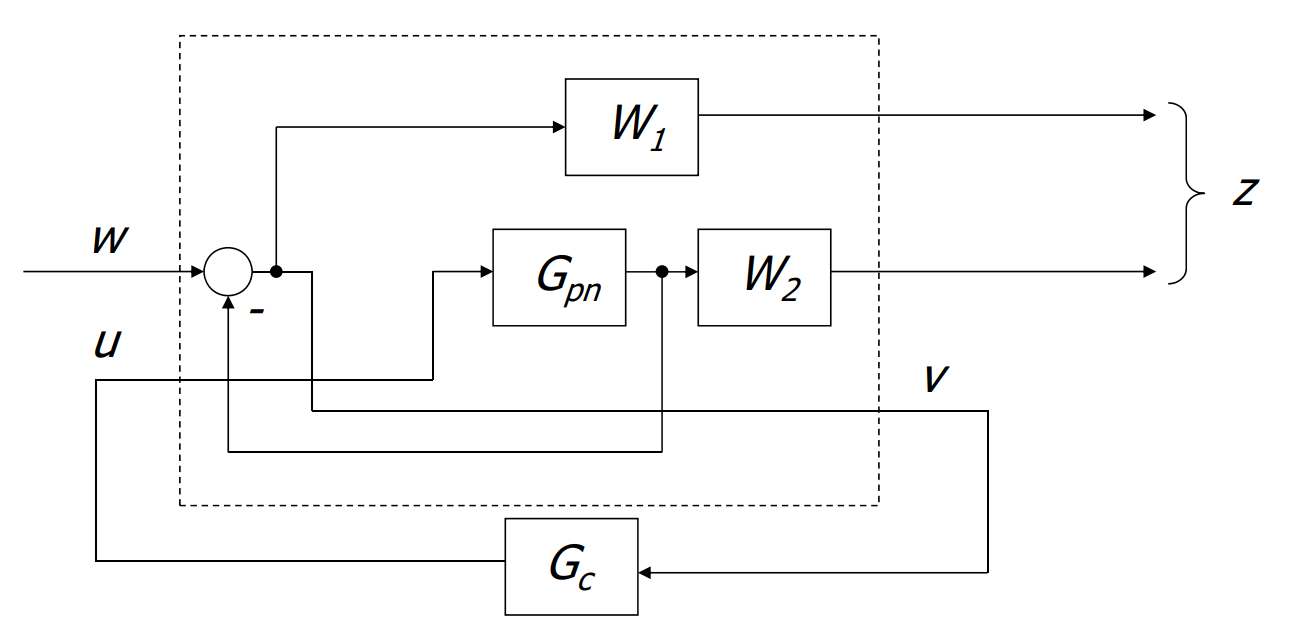
\includegraphics[width=0.75\textwidth]{mixed-sensitivity-problem.png}
    \caption{The scheme of the generalized plant for a mixed sensitivity problem}
\end{figure}

Consider the system described by the following equations (i.e. the generalized plant $M$ when only the input $u$ and the output $v$are considered)
\[
\begin{cases}
    \dot{x}_M = A x_M + B_2 u\\
z = C_1 x_M + D_{12} u\\
v = C_2 x_M + D_{22} u
\end{cases}
\]
Assumptions I requires that all the eigenvalues of the unobservable and uncontrollable part of this system are stable.\\

It easily seen from the block diagram of $M$ that all the modes of $A$ are controllable from $u$, while the modes of $A$ related poles of $W1$ and $W2$ are not observable from $v$.\\

Therefore, we have the following result:
\subsection{Result) Internal stability of the generalized plant $M$}
Consider the mixed sensitivity problem. The generalized plant 
$M$ can be internally stabilized by an LTI controller $G_c$ having input $v$ and input $v$ and output $u$ \textbf{if and only if} $W_1$ and $W_2$ are stable transfer functions.\\

Remark: This result requires that $W_1$ and $W_2$ are stable transfer functions. However, we know that some common performance requirements on the steady-state response to polynomial reference signals and disturbances lead to an unstable weighting function $W_1$ (due to the presence of one or more poles at $s = 0$)\\

Now, assume that the performance requirements are such that the weighting function $W_1$ has $\nu + p$ poles at $s = 0$.\\

In order to satisfy assumption I, we replace $W_1$ in the generalized plant $M$ with a new weighting function $W_1^{*}$ obtained as follows\\
\[
W_1^{*} = W_1 \frac{s^{\nu+p}}{(s + \lambda^{*})^{\nu + p}}
\]

So the modified $W_1$, $W_1^{*}$ is going to be as follows:

\begin{figure}[H]
    \centering
    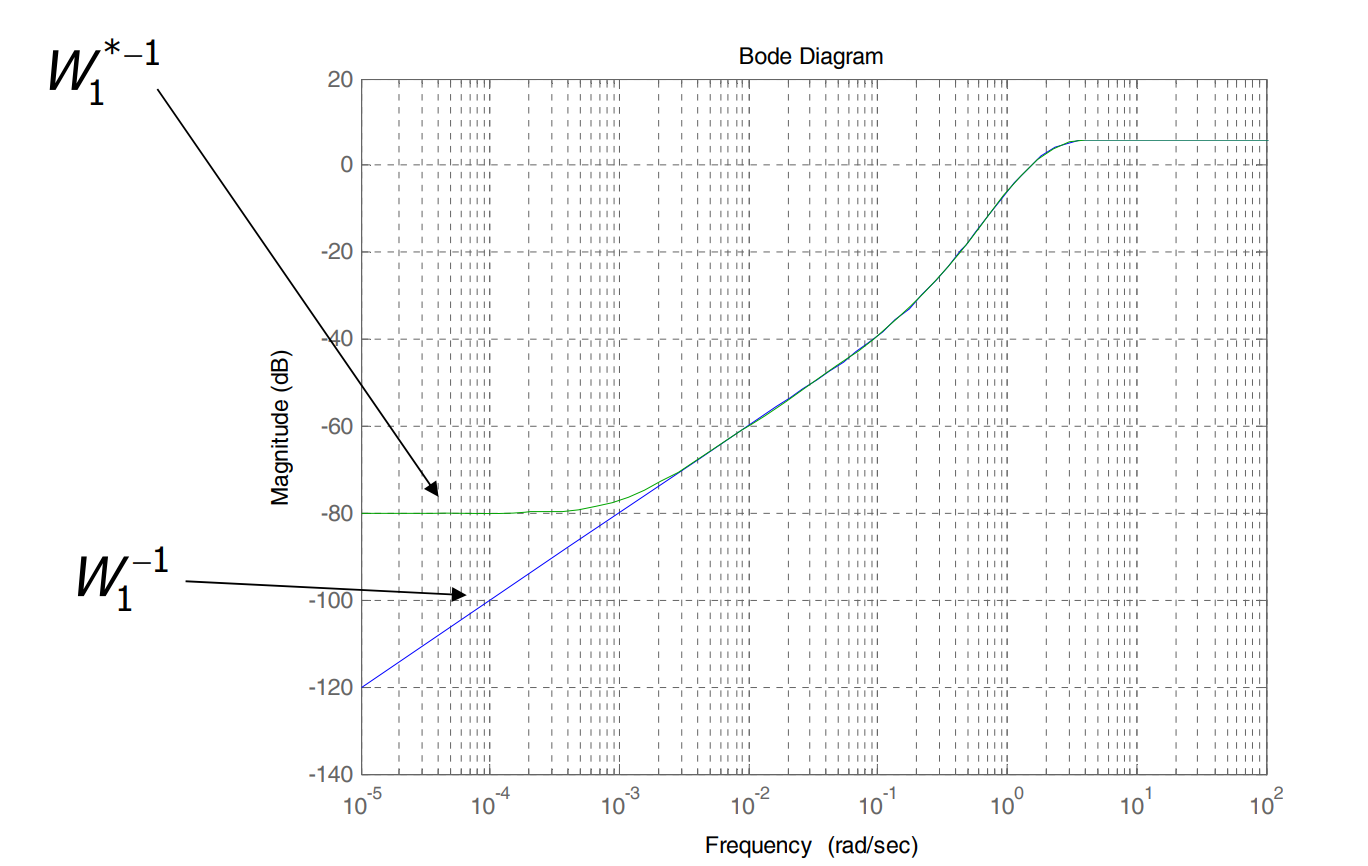
\includegraphics[width=0.75\textwidth]{modified-w1.png}
    \caption{The plot of the $W_1$ and its modified version,$W_1^{*}$}
\end{figure}


\begin{factbox}[About this kind of pole substitution]
Since the pole that is to be substituted has a frequency less than the cross over frequency of the weighting function, in this case a pole with frequency 0, in order no to modify the crossover frequency of the modified transfer function, the substitution should be sond in this zero-pole form $s + \lambda$, and not the dc-gain form. In this way, the dc-gain of the transfer function is adjusted such that the crossover frequency of the system does not change.\\

If the substitution or the cancellation is to be done on a pole or zero with a cutting frequency more than the crossover frequency, since the removal, or substitution does not affect the crossover frequency, there is no need so that the dcgain is modifies, so this operation can be done in the dcgain form ($1 + \frac{s}{\lambda^{*}}$), this is usefull for reducing the order of the controller obtained by the optimizer.
\end{factbox}

\newpage

\subsubsection{Need for modification of $W_2$}
$W_2$ is stable, but not proper, so we face a problem while creating the generalized plant in the Simulink, since it is not allowed to use uncausal blocks in Simulink. Hence, $W_2^{*}$ used in the Simulink block of the generalized plant $M$ is as follows:
\[
W_2^{*} = \frac{1}{T_{p0}}
\]
Now, in order to retreive the original form of $W_2$, in the command line the zeros are augmented,\\

\texttt{sderiv(M,2,[\textit{'the polynomial form of the derivator'}])} \\

where, 2 refers to the output channel on which the operation of derivative needs to be imposed, e.g. in the following $W_2$
\[
W_T = \frac{(1 + \frac{s}{p})(1 + \frac{s}{p})}{T_{p0}}
\]
\[
W_2^{*} = \frac{1}{T_{p0}}
\]
and in the command line, it need to be writen
\texttt{M = sderiv(M,2,[1/p 1])}
\texttt{M = sderiv(M,2,[1/p 1])}

\begin{factbox}[Experience]
According to the professor's experience, the optimizer return a better result for a generalized plant with real poles in the $W_2$. Therefore, another modification before doing the aforementioned modification is to make $W_2$ with real poles. 
\end{factbox}

\begin{QandAbox}[commands regarding $W_1^{*}$ and $W_2^{*}$]
Consider these two transfer functions as the nubs in order to obtain a better controller in terms of performance and simplicity. \\

For example, if the resultant loop function is not as fast as it is expected, by increasing the crossover frequency of $W_1$, one can force the optimizer to return a controller which results in a faster system, or if the overshoot need to be modified, the higher of $W_1$ or $W_2$ can be modified.
\end{QandAbox}

The following MATALB codes is to be used here:
\begin{itemize}
    \item \texttt{[Am, Bm, Cm, Dm] = linmod('simulink\_generalized\_plant')}\\
    \item \texttt{M = ltisys(Am, Bm, Cm, Dm)}\\
  
    \item If zeros need to be appended:\\
    \texttt{M = sderiv(M, 2, [1/p 1])}\\
    \texttt{M = sderiv(M, 2, [1/p 1])}\\
    
    \item \texttt{[g\_opt, Gc\_mod] = hinflmi(M, [1\ 1], 0, 0.01, [0\ 0\ 0])}\\
    \begin{itemize}
        \item \texttt{[1\ 1]} represents the number of inputs and outputs of the controller.
        \item \texttt{0} specifies gamma optimal (minimum achievable gamma).
        \item \texttt{0.01} defines the relative accuracy of the gamma optimum.
        \item \texttt{[0\ 0\ 0]} are optional parameters.
    \end{itemize}
    
    \item \texttt{[Ac, Bc, Cc, Dc] = ltiss(Gc_mod)}\\
    \item \texttt{Gc_mod = ss(Ac, Bc, Cc, Dc)}
\end{itemize}
Use minreal, to make sure cancellations are done.

